\documentclass[10pt, compress]{beamer}

\usetheme{m}

\usepackage{booktabs}
\usepackage[scale=2]{ccicons}
\usepackage{minted}
\usepackage{graphicx}

\DeclareMathOperator{\Hash}{Hash}
\DeclareMathOperator{\Number}{Number}

\usepgfplotslibrary{dateplot}

\usemintedstyle{trac}

\title{ParKazoo}
\subtitle{Implementing a partitioned ZooKeeper using Kazoo}
\date{\today}
\author{Arjun Naik}
\institute{TU Dresden}

\begin{document}

\maketitle

\section{Introduction}

\begin{frame}[fragile]
    \frametitle{Coordination in Distributed Systems}
    \begin{itemize}
        \item Configuration data
        \item Asynchronous Operation
        \item Partitions possible
        \item Redundancy
        \item Fault-Tolerance
    \end{itemize}
\end{frame}

\begin{frame}[fragile]
    \frametitle{ZooKeeper}
    A service for coordinating processes of distributed applications.
    \begin{quote}
        ZooKeeper aims to provide a simple and high performance kernel for building more complex
        coordination primitives at the client. 
    \end{quote}
\end{frame}

\begin{frame}[fragile]
    \frametitle{ZooKeeper Architecture}
    \begin{figure}[ht!]
        \centering
        \includegraphics[width=100mm]{images/ZKArchWithoutBG.png}
    \end{figure}
\end{frame}

\begin{frame}
    \frametitle{Problems with ZooKeeper}
    \begin{itemize}
        \item Consensus is slow
        \item Read throughput increases as more servers are added
        \item Write throughput decreases with consensus size.
        \item Hence trade-off between read and write performance.
    \end{itemize}
\end{frame}

\begin{frame}[fragile]
    \frametitle{Solution: ParKazoo}
    \begin{itemize}
        \item Use multiple ZK clusters(Ensemble)
        \item Tree structure is distributed
        \item Host cluster of node depends on the parent path
        \item All siblings on same cluster
    \end{itemize}
    

    \textbf{ParKazoo Features}
    \begin{itemize}
        \item Pure Python Implementation
        \item Supports Gevent (single threaded IO Loop)
        \item Implements many of the popular recipes.
    \end{itemize}
\end{frame}

\section{Approach}
\begin{frame}[fragile]
    \frametitle{Partitioned Architecture: Diagram}
    \begin{figure}[ht!]
        \centering
        \includegraphics[width=70mm]{images/ParKazooArchWithoutBG.png}
        \caption{ParKazoo Ensemble \label{overflow}}
    \end{figure}
\end{frame}

\begin{frame}[fragile]
    \frametitle{Partitioned Architecture}
    \begin{itemize}
        \item Multiple Clusters
        \item Single Ensemble
        \item Every client connects to every Cluster
        \item Connections are distributed over Clusters
        \item Linear speedup can be achieved.
    \end{itemize}
\end{frame}

\begin{frame}[fragile]
    \frametitle{Assigning Node to cluster}
    Path of parent is used to calculate the destionation cluster.
    \begin{equation}
        Cluster_{Destination} = \Hash(Path_{Parent})\bmod \Number(Clusters)
    \end{equation}
    Sibling nodes get mapped to the same cluster.
\end{frame}

\begin{frame}
    \frametitle{Caveats and Workarounds}
    \begin{itemize}
        \item Primary Order cannot be preserved.
        \item Most Recipes require Primary Order
    \end{itemize}
    \subsection{Work Around}{
        \textbf{Work Around}
        Recipes require primary order on siblings. ParKazoo mapping scheme maps siblings to same cluster and hence primary order is preserved between them
    }
\end{frame}

\section{Measurements}
\begin{frame}
    \frametitle{Throughput}
    \begin{figure}
    \begin{tikzpicture}
      \begin{axis}[
        xlabel={Time},
        ylabel={Requests},
        msimpleplot,
        width=0.9\textwidth,
        height=6cm,
        legend columns=2,
        enlarge y limits=0.02,
      ]

        \addplot table[x=column1,y=column2] {data/zookeeper_sampled.dat}; 
        \addplot+ table[x=column1,y=column2] {data/parkazoo_sampled.dat}; 
        \legend {ZooKeeper, ParKazoo}
      \end{axis}
    \end{tikzpicture}
  \end{figure}
\end{frame}

\begin{frame}
    \frametitle{Performance}
    \begin{figure}
    \begin{tikzpicture}
      \begin{axis}[
        xlabel={Clients},
        ylabel={Writes},
        mlineplot,
        width=0.9\textwidth,
        height=6cm,
        legend columns=2,
        enlarge y limits=0.02,
      ]

        \addplot table[x=column1,y=column2] {data/parkazoo_performance.dat}; 
        \addplot+ table[x=column1,y=column2] {data/zookeeper_performance.dat};
        \legend {ParKazoo, ZooKeeper}
      \end{axis}
    \end{tikzpicture}
  \end{figure}
\end{frame}


\section{Next Steps}
\begin{frame}[fragile]
    \frametitle{Consistency Levels}
    \begin{itemize}
        \item Weak consistency
        \item No primary order
        \item No Transaction support
        \item Significant speedup
    \end{itemize}
\end{frame}

\begin{frame}
    \frametitle{Async Support}
    \begin{itemize}
        \item Handlers for Gevent.
        \item Implement async operations.
    \end{itemize}

\end{frame}

\begin{frame}
    \frametitle{Improve Testing}
    \begin{itemize}
        \item Multinode sampled tests
        \item Testing with barriers
        \item Sampling through events
    \end{itemize}
\end{frame}

\plain{Questions?}

\section{Auxilliary Slides}

\begin{frame}
    \frametitle{Related Software}
    \begin{itemize}
        \item Paxos (Leslie Lamport)
        \item Chubby (by Google)
        \item Etcd, Doozerd (Written in Go)
        \item Raft (Simpler Protocol)
        \item Consul, Serf(Built with Raft)
    \end{itemize}
\end{frame}

\begin{frame}[fragile]
    \frametitle{Primary Order}
    \begin{itemize}
        \item All operations from client are executed in order.
        \item The write operations are ordered but reads are not.
    \end{itemize}
\end{frame}

\subsection{ParKazoo Operations}
\begin{frame}[fragile]
    \frametitle{Creating a Node}
    \begin{itemize}
        \item Check if the parent exists on its cluster.
        \item Check if parent is ephemeral
        \item If everything ok, then create the Node.
    \end{itemize}
    \begin{figure}[ht!]
        \centering
        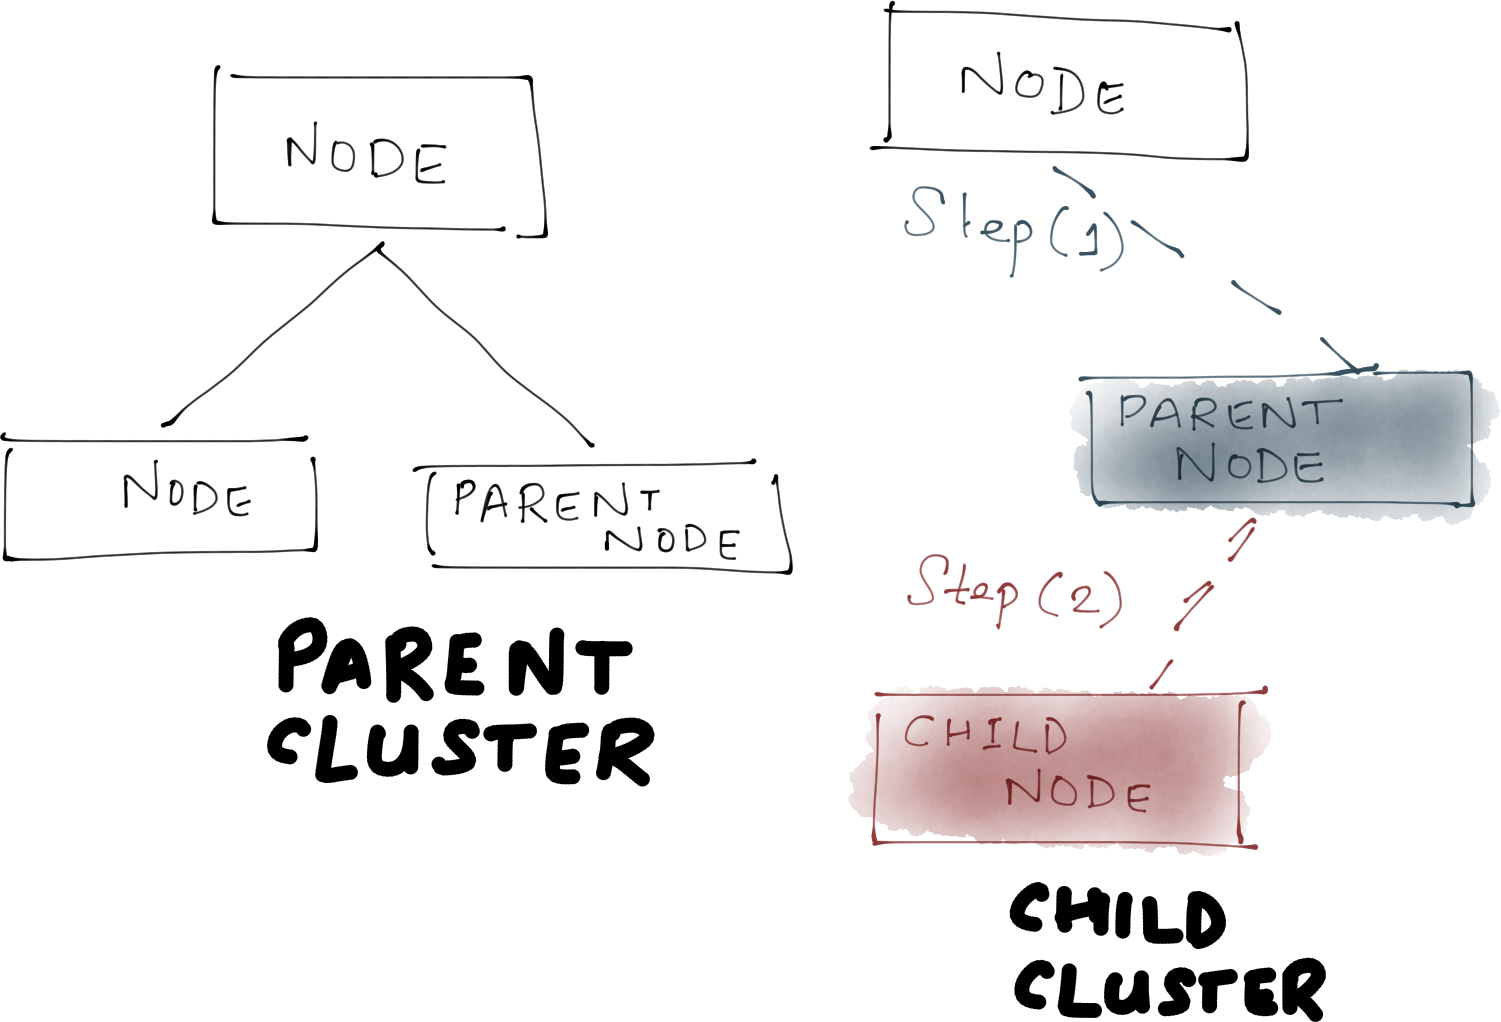
\includegraphics[width=60mm]{images/ParKazooCreate.png}
    \end{figure}
\end{frame}

\begin{frame}[fragile]
    \frametitle{Getting Children of Node}
    \begin{itemize}
        \item All children of Node on single cluster.
        \item Check if node exists
        \item Check if the path exists on children cluster.
        \item If not create it, so that watches can be left.
    \end{itemize}
\end{frame}

\begin{frame}[fragile]
    \frametitle{Deleting a Node}
    \begin{itemize}
        \item Delete can be recursive.
        \item Then delete from all clusters.
        \item If not recursive, then check if node has children.
    \end{itemize}
\end{frame}

\end{document}
